%Sidenote from Angie: Green text after a percentage sign includes notes to the LaTeX code, useful tips and tricks I thought you might need ⁠— feel free to read them for extra info on this template.

%~~~~~~~~~~~~~~~~~~~~~~~~~~~~~~~~~~~~~~~~~~~~~~~~~~~~~~~%
% Changelog 7.21: Lab now moving from remote learning to physical laboratory, please ignore any comments after '% OLD TEXT IGNORE:'
%Changelog 10.21: Fixed the formatting of RSC referencing style 
%Changelog 1.22: Reviewed before the start of Semester 2, fixed some wording/clarification issues
%Changelog 5.22: Reviewed after semester 2, fixed some wording/clarification issues, removed OLD TEXT
%~~~~~~~~~~~~~~~~~~~~~~~~~~~~~~~~~~~~~~~~~~~~~~~~~~~~~~~%

\documentclass[twocolumn]{article} %sets the type of the document that you compile, for just now it is an article - specifically one with a two-column formatting

%~~~~~~~ Packages ~~~~~~~~~%
% Please don't be scared by the chunk of code below, these are just some handy tools that make using LaTeX easier, you can read more on your own time, for example here: https://www.latex-tutorial.com/tutorials/packages/
%\usepackage{amsmath}
% \usepackage{caption}
% \usepackage{subcaption}
\usepackage[utf8]{inputenc} %helps interpret unicode, non ASCII characters
\usepackage[T1]{fontenc} %makes font compatible with more non-ASCII characters
\usepackage[english]{babel} %allows the use of special characters and also translates some elements within the document. This package also automatically activates the appropriate hyphenation rules for the language you choose
\usepackage{ifpdf,amsmath,amsthm,amssymb,amsfonts,newtxtext,newtxmath} %helps formatting math & keeps it looking tidy when compiling PDFs
\usepackage{array,graphicx,dcolumn,multirow,abstract,hanging} %makes tables compile properly & helps with nice table formatting
\usepackage{subcaption}
\usepackage[font={it,footnotesize},labelfont=bf]{caption} %makes captions nicer
\usepackage[hyperfootnotes=false,breaklinks=true,hidelinks]{hyperref} %formats hyperlinks
%\hypersetup{colorlinks=false,} %formats hyperlinks
\usepackage{float} %improves the interface for defining floating objects such as figures and tables
\urlstyle{same} %formats urls
\usepackage{url} %formats urls
\usepackage[version=4]{mhchem} %helps format chemical formulae see more info at https://anorien.csc.warwick.ac.uk/mirrors/CTAN/macros/latex/contrib/mhchem/mhchem.pdf
\usepackage{siunitx} %formats SI units see more info at http://www.bakoma-tex.com/doc/latex/siunitx/siunitx.pdf
\usepackage{color,soul} %allows for highlighting text
\usepackage[super,sort&compress,comma]{natbib}  % use natbib
\setlength{\bibsep}{0pt plus 0.3ex} % set spacing of bibliography
\usepackage{booktabs} % \toprule \midrule \bottomrule \cmidrule(lr){a-b}
%\usepackage{capt-of}
% define centered and ragged columns:
\newcolumntype{L}[1]{>{\raggedright\arraybackslash }p{#1}} % can use m{}
\newcolumntype{C}[1]{>{\centering\arraybackslash }p{#1}}
\newcolumntype{R}[1]{>{\raggedleft\arraybackslash }p{#1}}
\newcolumntype{d}[1]{D{.}{.}{#1}} % d{3.2} for 3 places on l, 2 on r
\newcommand{\mc}{\multicolumn}
\topmargin=-.3in \oddsidemargin=-.1in \evensidemargin=-.1in \textheight=9in \textwidth=6.8in
\setlength\tabcolsep{1mm}
\setlength\columnsep{8mm}
\setlength\abovecaptionskip{.5ex}
\setlength\belowcaptionskip{.5ex}
\setlength\belowbottomsep{.3ex}
\setlength\lightrulewidth{.04em}
\renewcommand\arraystretch{1.2}
\renewcommand{\topfraction}{1}
\renewcommand{\textfraction}{0}
\renewcommand{\floatpagefraction}{.9}
\renewcommand{\thefootnote}{\roman{footnote}}
% \renewcommand{\baselinestretch}{1.00} \large\normalsize % for fixing spaces
\widowpenalty=1000
\clubpenalty=1000
\setlength{\parskip}{0ex}
\let\tempone\itemize
\let\temptwo\enditemize
\let\tempthree\enumerate
\let\tempfour\endenumerate
\renewenvironment{itemize}{\tempone\setlength{\itemsep}{0pt}}{\temptwo}
\renewenvironment{enumerate}{\tempthree\setlength{\itemsep}{0pt}}{\tempfour}
%the above is the formatting setup for keeping the two-column article and tables working nicely, feel free to tinker with it, but I suggest only doing so once you know what you're doing with LaTeX
%~~~~~~~~~~~~~~~~~~~~~~~~~~%

%!!!!!!!!!!!!!!!!!!!!!!!!!!!!!!!!!!!!!!%
% REPORT STARTS HERE %

%\date{} %if you don't want the date to show up in your report, uncomment this (=remove the percentage symbol at the start of the line)
\setcounter{page}{1} % starts counting pages from the first
\title{Bioremediation previous cases} % change to an actual title for your report!
\author{Qianrui Li}

\begin{document}
\twocolumn[ %this command makes your title and abstract both be one column only
\vspace{-.5in}
\maketitle
\centering
\vspace{-0.3in}
\section*{Abstract}
{\large 
This summary shows the previous cases of bioremediation. 

}
\vspace{0.4in}
]
%\setlength{\baselineskip}{12pt plus.2pt}


\section{case 1} % example of a heading

\textbf{Nitro}\cite{nitrobioremed}\\
In this study, nitrate bioremediation in groundwater impacted with gasoline containing 25\% ethanol was evaluated during 32 months in a field experiment. By means of mass and spatial distribution analysis of the dissolved compounds, biostimulation was found to have a positive influence on ethanol and BTEX biodegradation, and prevented the formation of highly reducing zones (90\% of values were higher than + 100 mV) and BTEX and ethanol plume migration in the monitoring area. Results indicate that nitrate biostimulation is a highly efficient alternative in remediating groundwater impacted by gasohol.
\\ 

\section{case 2}
\textbf{Nitro2}\cite{nitro2}\\
The purpose of the present study was to investigate possible methods to enhance the rate of aerobic biodegradation of hydrocarbons (ex-situ treatments). In this work, the bioremediation processes were applied to a sandy soil with a high level of contamination originated from the leakage of a diesel oil underground storage tank at a petrol station. Laboratory scale experiments (Bartha biometer flasks) were used to evaluate the biodegradation of the diesel oil. Enhancement of biodegradation was carried out through biostimulation (addition of nitrogen and phosphorus solutions or Tween 80 surfactant) and bioaugmentation (bacterial consortium isolated from a landfarming system). To investigate interactions between optimizing factors, and to find the right combination of these agents, the study was based on full factorial experimental design. Efficiency of biodegradation was simultaneously measured by two methods: respirometric (microbial CO2 production) and gas chromatography. Acute toxicity tests with Daphnia similis were applied for examination of the efficiency of the processes in terms of the generation of less toxic products. Results showed that all bioremediation strategies enhanced the natural bioremediation of the contaminated soil and \textbf{the best results were obtained when treatments had nutritional amendment}. Respirometric data indicated a maximum hydrocarbon mineralization of 19.8\%, obtained through the combination of the three agents, with a total petroleum hydrocarbons (TPH) removal of 45.5\% in 55 days of treatment. At the end of the experiments, \textbf{two predominant bacteria species were isolated and identified (Staphylococcus hominis and Kocuria palustris)}.
\\

\section{case 3}
\textbf{Bioaugmentation}\cite{bioaugmentation}\\
Bioaugmentation can occur either by the use of a single strain microorganism or between different microorganisms (fungi and bacteria). In the present study, we carefully evaluated these two bioaugmentation forms on the degradation of total petroleum hydrocarbon (TPH) in gasoline polluted soil. Microbial activity indexed by dehydrogenase (DHA) assay and effect of pH on biodegradation were also measured. After 8 week incubation, all the studied systems showed varying degree of TPH removal from the gasoline polluted soil. Highest percentage of degradation (75.70\%) was observed in Micrococcus luteus, 71.10\% in Rhizopus arrhizus and 66.40\% in the consortium though removal efficiencies were not statistically different among the bioaugmentation options but differed significantly with the control at 
. The natural attenuation (control) system had the least TPH removal efficiency (54.04\%). The study reported that bioaugmentation involving microbial consortium resulted in initial accelerated biodegradation rates. Fungi bioaugmented systems had low pH condition throughout the experiment. Results of microbial dynamics showed that population density of total heterotrophic microorganisms were higher than actual gasoline degraders and studies using kinetic parameters supported that significant gasoline hydrocarbon removal occurred in the bioaugmentation systems.

\begin{figure}[H]
    \centering
    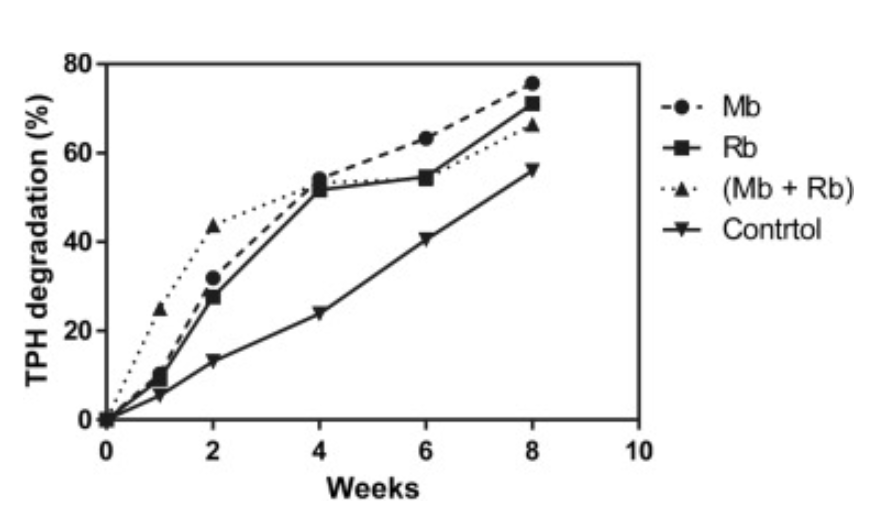
\includegraphics[width=\columnwidth]{bioau.png}
    \caption{TPH removal efficiency within the study period. Mb—Micrococcus luteus, Rb—Rhizopus arrhizus, Mb + Rb—Microbial consortium (Micrococcus luteus and Rhizopus arrhizus), Control—No added microorganisms.}
\end{figure}

\section{case 4}
\textbf{Adding poultry litter, coir pith and rhamnolipid biosurfactant}\cite{4}\\
The aim of the present study was to find methods for enhancing rates of hydrocarbon biodegradation in gasoline contaminated soil by ex situ bioremediation. Red soil (RS) was treated with gasoline-spilled soil (GS) from a gasoline station and different combinations of amendments were prepared using (i) mixed bacterial consortium (MC), (ii) poultry litter (PL), (iii) coir pith (CP) and (iv) rhamnolipid biosurfactant (BS) produced by Pseudomonas sp. DS10-129. The study was conducted for a period of 90 days during which bacterial growth, hydrocarbon degradation and growth parameters of Phaseolus aureus RoxB including seed germination, chlorophyll content, shoot and root length were measured. Approximately 67\% and 78\% of the hydrocarbons were effectively degraded within 60 days in soil samples amended with RS + GS + MC + PL + CP + BS at 0.1\% and 1\%. Maximum percentage of seed germination, shoot length, root length and chlorophyll content in P. aureus were recorded after 60 days in the above amendments. Further incubation to 90 days did not exhibit significant improvements. Statistical analysis using analysis of variance (ANOVA) and Duncan's multiple range test (DMRT) revealed that the level of amendments, incubation time and combination of amendments significantly influenced bacterial growth, hydrocarbon degradation, seed germination and chlorophyll content at a 1\% probability level. All tested additives MC, PL, CP and rhamnolipid BS had significant positive effects on the bioremediation of GS.

Approximately 67\% and 78\% of the hydrocarbons were effectively degraded within 60 days in soil samples amended with RS + GS + MC + PL + CP + BS at 0.1\% and 1\%.

\begin{figure}[H]
    \centering
    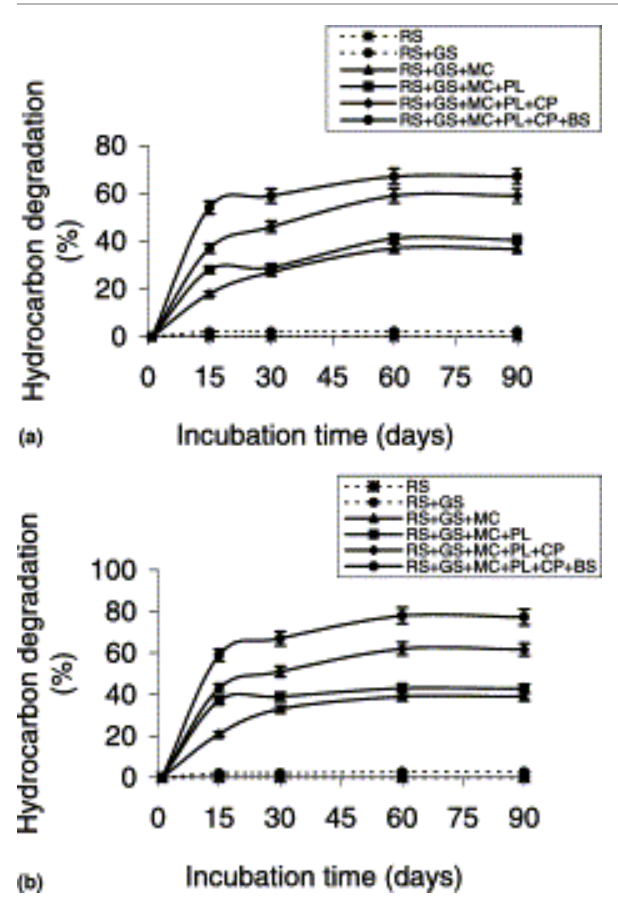
\includegraphics[width=\columnwidth]{soil.png}
    \caption{Hydrocarbon degradation during various treatments at regular intervals in GS. (a) Results of the treatment with 0.1\% amendments. (b) Results of the treatment with 1.0\% amendments.}
\end{figure}

\section{case 5}
\textbf{feasibility of bioremediation of petroleum hydrocarbon contaminated soil}\cite{5}\\
Laboratory and field pilot studies were carried out on the bioremediation of soil contaminated with petroleum hydrocarbons in the Borhola oil fields, Assam, India. The effects of aeration, nutrients (i.e. nitrogen and phosphorus) and inoculation of extraneous microbial consortia on the bioremediation process were investigated. The beneficial effects of these parameters on the bioremediation rate were realised equally in laboratory and field pilot tests. The field tests revealed that up to 75\% of the hydrocarbon contaminants were degraded within 1 year, indicating the feasibility of developing a bioremediation protocol. A complementary computer simulation study was carried out to enhance the understanding of the basic processes and the rate determining factors for bioremediation under the practically relevant conditions of Borhola oil fields. The simulations indicated that due to the high initial contaminant concentrations, the bioremediation process was restricted mostly to the macropores of the system within the period of 1 year and had not penetrated into the soil aggregates sufficiently. Certain shortcomings of the model have been identified and possible refinements suggested.

\textbf{The field pilot study showed that by applying nutrient and microbe enriched solution, the crude oil components were reduced under aerated conditions by 75\% within a time span of 1 year. }This observation is supplemented by a laboratory enumeration of adequate soil microbial and chemical properties, which can be exploited for designing a large-scale process system for field application. 

\section{case 6}
\textbf{agricultural wastes for bioremediation of oil-contaminated soil}\cite{6}\\
Agricultural wastes, such as wheat bran and swine wastewater, were used for bioremediation of oil-contaminated soil. Two optimised strains that could degrade oil efficiently were selected. The result showed that the best ratio of strain A to strain B was 7:3. Swine wastewater could be a replacement for nitrogen source and process water for bioremediation. \textbf{Under the optimal medium, the oil degradation rate reached 68.27 after 40 d.} The urease, catalase, and dehydrogenase activities in oil-contaminated soil all increased, and the microbe quantity increased significantly with manual composting. These investigations might lay a foundation for reducing the pollution of agricultural wastes, exploring a late model for bioremediation of oil-contaminated soil.
\begin{figure}[H]
    \centering
    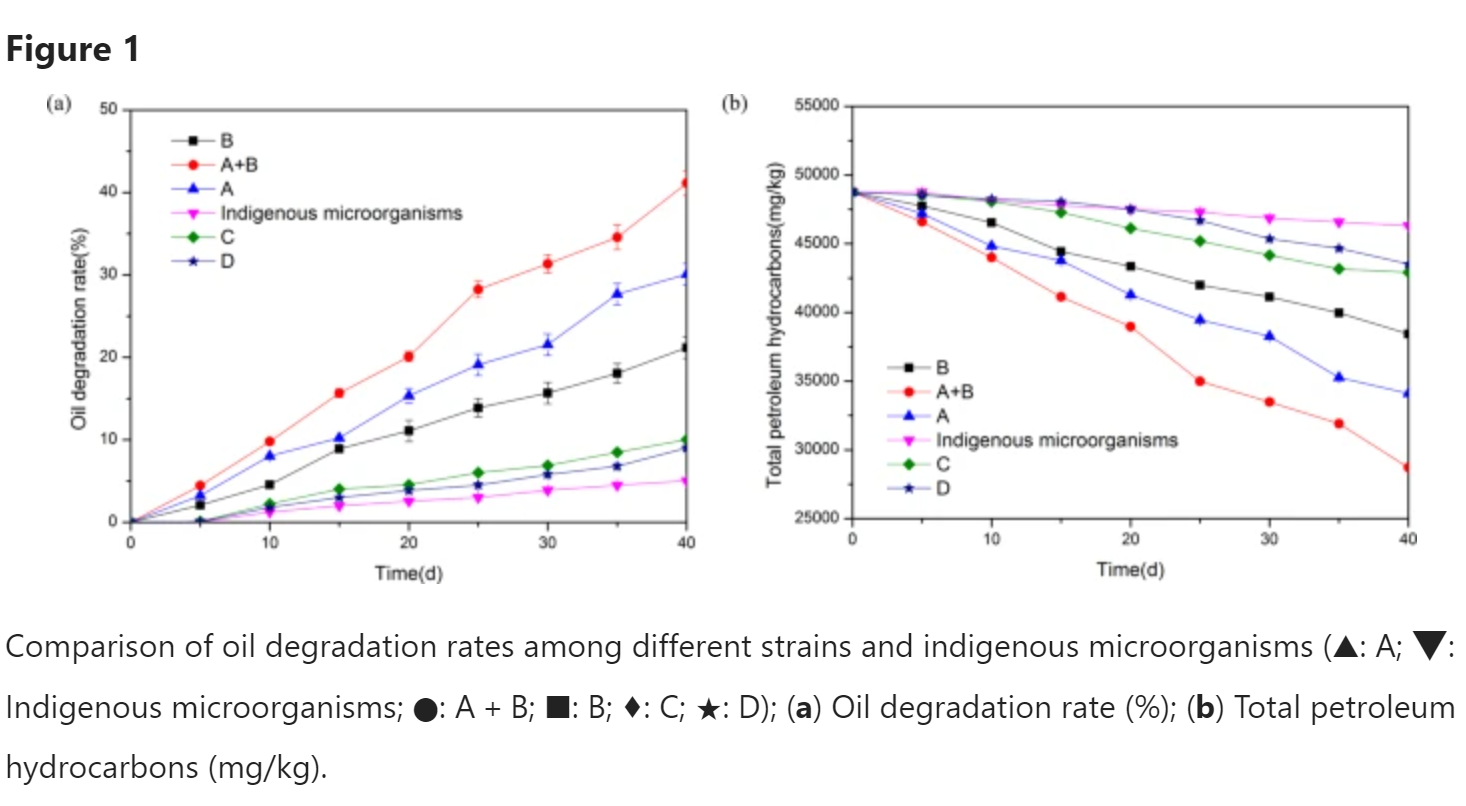
\includegraphics[width=\columnwidth]{6.png}
    \caption{Comparison of oil degradation rates among different strains and indigenous microorganisms}
\end{figure}


\section{case 7}
\textbf{comparison among different bioremediation}\cite{7}\\
Increasing industrialisation, continued population growth and heavy demand and reliance on petrochemical products have led to unprecedented economic growth and development. However, inevitably this dependence on fossil fuels has resulted in serious environmental issues over recent decades. The eco-toxicity and the potential health implications that petroleum hydrocarbons pose for both environmental and human health have led to increased interest in developing environmental biotechnology-based methodologies to detoxify environments impacted by petrogenic compounds. Different approaches have been applied for remediating polluted sites with petroleum derivatives. Bioremediation represents an environmentally sustainable and economical emerging technology for maximizing the metabolism of organic pollutants and minimizing the ecological effects of oil spills. Bioremediation relies on microbial metabolic activities in the presence of optimal ecological factors and necessary nutrients to transform organic pollutants such as petrogenic hydrocarbons. Although, biodegradation often takes longer than traditional remediation methods, the complete degradation of the contaminant is often accomplished. Hydrocarbon biodegradation in soil is determined by a number of environmental and biological factors varying from site to site such as the pH of the soil, temperature, oxygen availability and nutrient content, the growth and survival of hydrocarbon-degrading microbes and bioavailability of pollutants to microbial attack. In this review we have attempted to broaden the perspectives of scientists working in bioremediation. We focus on the most common bioremediation technologies currently used for soil remediation and the mechanisms underlying the degradation of petrogenic hydrocarbons by microorganisms.

\textbf{natural attenuation}\\
Sometimes even better than bioaugmentation and biostimulation.

\textbf{bioaugmentation}\\
When the indigenous microbes are not enough, we can add some microbes to the soil to help the degradation.
The rationale behind bioaugmentation is that the introduction of hydrocarbon degrading microorganisms into polluted soil improves the biodegradative capacity of the indigenous population. 

\textbf{biostimulation}\\
There exists extensive literature that have reported that high concentrations of petroleum hydrocarbon, containing around 80\% carbon can lead to a rapid reduction in the concentration of inorganic nutrients present in the soil (e.g. nitrogen and phosphorus)\cite{7.2}\\
However care must be taken in the amount of nutrients added; for example the addition of excess quantities of nitrogen may result in inhibition of the soil microbial community.




\begin{figure}[H]
    \centering
    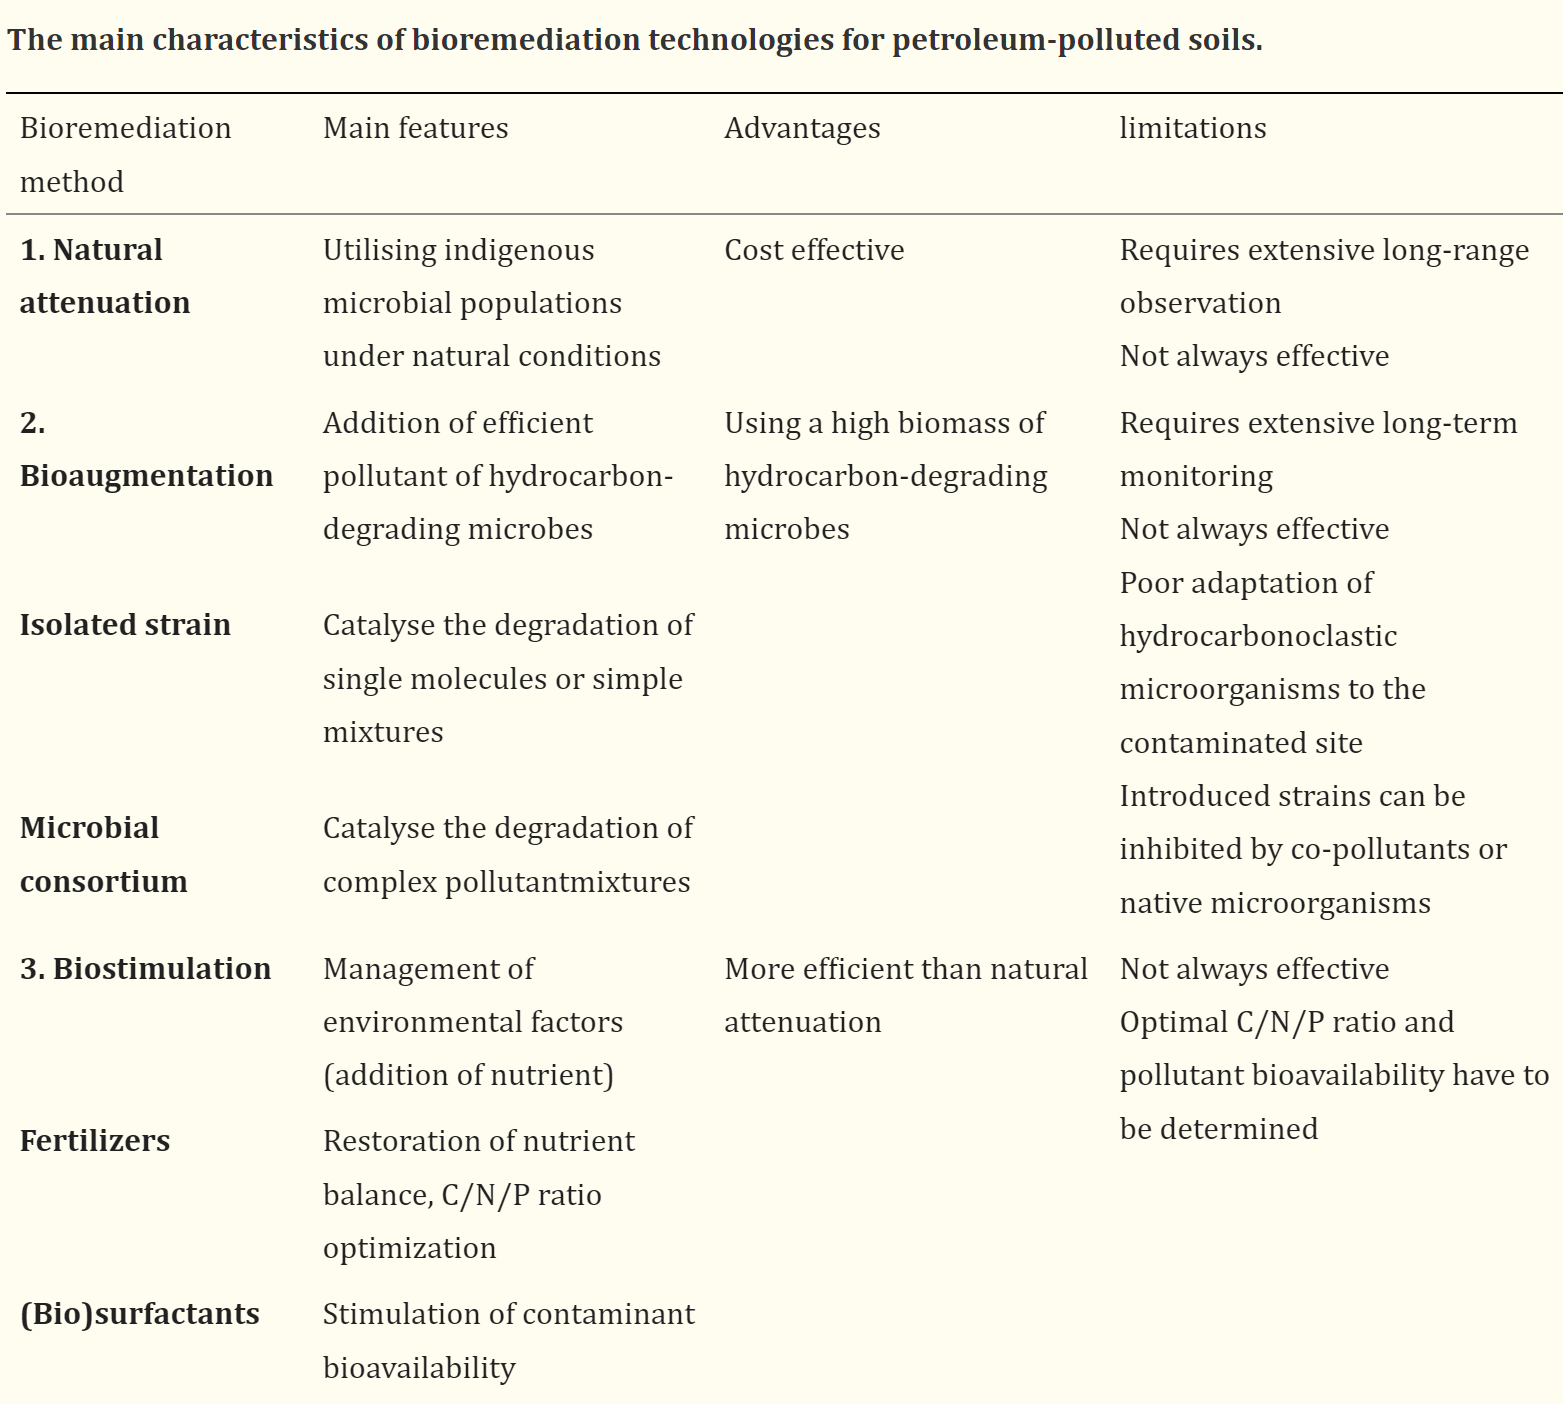
\includegraphics[width=\columnwidth]{7.png}
    \caption{Comparing different methods of bioremediation}
\end{figure}


EX3\cite{ex3}








\bibliography{ref} 
\bibliographystyle{rsc}

\end{document}

